\documentclass[a4paper,10pt]{article}
\usepackage[margin=30mm]{geometry}

% language
\usepackage[utf8]{inputenc}
\usepackage[english]{babel}
\usepackage{amsmath}
\usepackage{mathtools}
% colors
\usepackage{xcolor}
\definecolor{code_bg}{rgb}{0.95,0.95,0.92}

% code sections
\usepackage{listings}
\lstset{
  language=C,
  backgroundcolor=\color{code_bg},
  numbers=left,
  numbersep=5pt,
  numberstyle=\tiny\color{gray},
  captionpos=b,
  framexleftmargin=12pt,
  framextopmargin=2pt,
  framexbottommargin=2pt, 
  frame=tb, framerule=0pt,
  aboveskip=0pt,
  belowskip=1em,
  xleftmargin=4.5mm,
}

\usepackage{graphicx}         % includegraphics{}
\usepackage{float}            % H placement for figures
\usepackage{amsmath}          % matrix

\renewcommand\thesection{\Alph{section}}
\renewcommand\thesubsection{\Alph{section}\arabic{subsection}}

\newcommand{\task}[1]{{\bf #1}}

\usepackage{tikz}
\usetikzlibrary{calc}

\setlength{\parskip}{12pt}
\setlength{\parindent}{0pt}


\begin{document}
\begin{center}
  \textbf{\Huge TU Berlin Robotics WiSe 18/19} \\
  \textbf{\huge Lab Assignment \#2}
\end{center}

\vfill

\begin{figure}[H]
  \centering
  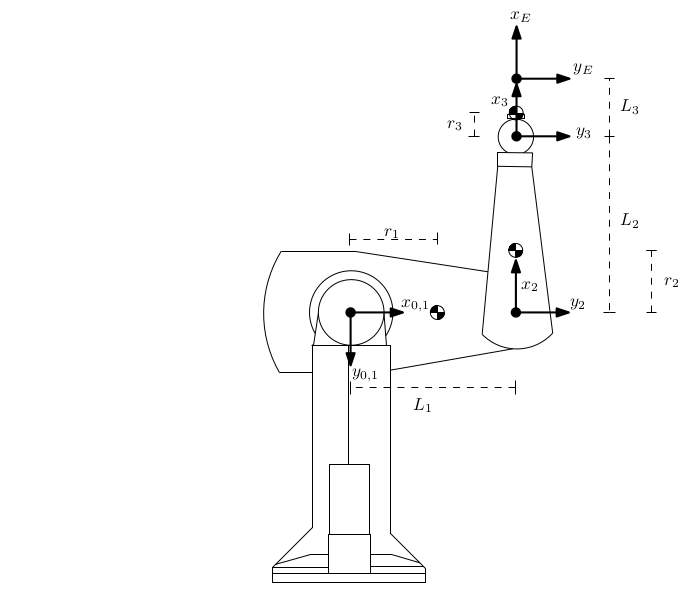
\includegraphics[scale=1.9]{img/robot_arm.png}
  \caption{RRR Puma in zero configuration}
\end{figure}

\begin{table}[h!]
  \begin{center}
    \begin{tabular}{c|c|c|c|c|c|c}
      Joint: & 1 & 2 & 3 & 4 & 5 & 6\\\hline
      $\tau_{max}$: & 97,6 Nm & 156,4 Nm & 89,4 Nm & 24,2 Nm & 20,1 Nm & 21,2 Nm
    \end{tabular}
    \caption{torque limits of the PUMA robot}
  \end{center}
\end{table}

\vfill

\begin{table}[h!]
  \begin{center}
    \begin{tabular}{rccccccccccc}
               ~          & \textbf{A1} & \textbf{A2} & \textbf{A3} & \textbf{(A4)} & \textbf{(B1)} & \textbf{B2} & \textbf{C1} & \textbf{C2} & \textbf{C3} & \textbf{C4} & \textbf{C5}\\\hline
      Jiaqiao Peng        &      ~      &      ~      &      ~      &       ~       &       x       &      x      &      x      &      ~      &      x      &      x      &      ~     \\\hline
      Benjamin Oesterle   &      x      &      x      &      x      &       x       &       x       &      x      &      x      &      x      &      x      &      x      &      ~     \\\hline
      Botond Péter Sléber &      x      &      x      &      x      &       x       &       x       &      x      &      ~      &      ~      &      ~      &      ~      &      ~     \\\hline
      Dhananjay Mukhedkar &      x      &      x      &      x      &       ~       &       x       &      ~      &      ~      &      ~      &      ~      &      x      &      ~     \\\hline
      
    \end{tabular}
    \caption{implementation table}
  \end{center}
\end{table}

\newpage

% -----------------------------------------------------------------------------

\section{Forward Kinematics}

\subsection{Transformation Between Frames}

\vspace{-6mm}Implemented in: \texttt{ForwardKinematicsPuma2D::computeTX\_Y()}

\begin{minipage}[b]{0.49\textwidth}
\centering
\begin{tabular}{c|c|c|c|c}
  $i$ & $\alpha_{i-1}$ & $a_{i-1}$ & $d_i$ &      $\theta_i$        \\\hline\hline
  1  &        0       &     0     &   0   &          $q_1$         \\
  2  &        0       &   $L_1$   &   0   & $q_2 - \frac{\pi}{2}$  \\
  3  &        0       &   $L_2$   &   0   &          $q_3$         \\
4(E) &        0       &   $L_3$   &   0   &           0
\end{tabular}
  
\vspace{1em}DH-parameters from assignment 1
\end{minipage}
\begin{minipage}[b]{0.49\textwidth}
\centering
${}^{i-1}_{i}T~=~\begin{bmatrix}
c\theta_i & -s\theta_i & 0 & \alpha_{i-1} \\
s\theta_ic\alpha_{i-1} & c\theta_ic\alpha_{i-1} & -s\alpha_{i-1} & -s\alpha_{i-1}d_i \\
s\theta_is\alpha_{i-1} & c\theta_is\alpha_{i-1} & c\alpha_{i-1} & c\alpha_{i-1}d_i \\
0 & 0 & 0 & 1 \\
\end{bmatrix}$

\vspace{1em}\hspace{1.8 cm}homogeneous transformation matrix
\end{minipage}

\textbf{Homogenous transformations between adjacent links:}

$\prescript{0}{1}{T}=
\begin{bmatrix} 
c_1 & -s_1  & 0 & 0\\
s_1 & c_1 & 0 & 0 \\
0 & 0 & 1 & 0 \\
0 & 0 & 0 & 1 
\end{bmatrix}
$

$
\prescript{1}{2}{T}=
\begin{bmatrix} 
s_2 & c_2 & 0 & L_1 \\
-c_2 & s_2 & 0 & 0 \\
0 & 0 & 1 & 0 \\
0 & 0 & 0 & 1
\end{bmatrix}
$

$\prescript{2}{3}{T}=
\begin{bmatrix} 
c_3 & -s_3 & 0 & L_2 \\
s_3 & c_3 & 0 & 0 \\
0 & 0 & 1 & 0 \\
0 & 0 & 0 & 1
\end{bmatrix}
$

$\prescript{3}{E}{T}=
\begin{bmatrix} 
1 & 0 & 0 & L_3 \\
0 & 1 & 0 & 0 \\
0 & 0 & 1 & 0 \\
0 & 0 & 0 & 1
\end{bmatrix}
$

\textbf{Forward kinematics for the end effector:}

$
\prescript{0}{E}{T}=\prescript{0}{1}{T} \cdot \prescript{1}{2}{T} \cdot \prescript{2}{3}{T} \cdot \prescript{3}{E}{T}=
\begin{bmatrix} 
s_{123} & c_{123} & 0 & c_1L_1 + s_{12}L_2 + s_{123}L3 \\
-c_{123} & s_{123} & 0 & s_1L_1 - c_{12}L_2 - c_{123}L_3 \\
0 & 0 & 1 & 0 \\
0 & 0 & 0 & 1
\end{bmatrix}
$

% -------------------------------------

\subsection{End Effector Position In Operational Space}

\vspace{-6mm}Implemented in: \texttt{ForwardKinematicsPuma2D::computeF()}

$
F(q)= \begin{pmatrix}x\\y\\\theta\end{pmatrix}=
\begin{pmatrix}
c_1L_1+s_{12}L_2+s_{123}L_3 \\
s_1L_1 - c_{12}L_2 - c_{123}L_3\\
q_1+q_2+q_3- \frac{\pi}{2}
\end{pmatrix}
$

% -------------------------------------

\subsection{Compute The End Effector Jacobian}

\vspace{-6mm}Implemented in: \texttt{ForwardKinematicsPuma2D::computeJ()}

$$
J(q) = \dfrac{\partial F(q)}{\partial q} = 
\begin{bmatrix}
-s_1L_1+c_{12}L_2+c_{123}L_3 & c_{12}L_2+c_{123}L_3 & c_{123}L_3 \\
~~~c_1L_1 + s_{12}L_2 + s_{123}L_3 & s_{12}L_2 + s_{123}L_3 & s_{123}L_3\\
1 & 1 & 1
\end{bmatrix} 
$$

% -------------------------------------

\subsection{Understanding The Jacobian Matrix And Pose Singularities}

\tikzstyle{joint} = [circle, fill=gray!80, inner sep=0.7mm]
\tikzstyle{velocity} = [->, >=stealth, red]

\subsection*{i) $q_1 = (0, 0, 0)^T$}

\begin{center}
\begin{minipage}{0.3\textwidth}
\centering
\begin{tikzpicture}[ultra thick, node distance=1.4cm]
  % joints
  \coordinate[joint]              (q1) at (0, 0);
  \coordinate[joint, right of=q1] (q2);
  \coordinate[joint, above of=q2] (q3);
  
  % base and end-effector
  \coordinate[below of=q1]                    (ba);
  \coordinate[above of=q3, node distance=7mm] (ee);
  
  % links
  \draw (ba) -- (q1);
  \draw (q1) -- (q2);
  \draw (q2) -- (q3);
  \draw (q3) -- (ee);
  
  % velocity vector
  \draw[velocity] (ee) -- ($(ee) + (1.0, -0.5)$);
\end{tikzpicture}

$\dot{q}_1 = (1, 0, 0)^T$
\end{minipage}
\begin{minipage}{0.3\textwidth}
\centering
\begin{tikzpicture}[ultra thick, node distance=1.4cm]
  % joints
  \coordinate[joint]              (q1) at (0, 0);
  \coordinate[joint, right of=q1] (q2);
  \coordinate[joint, above of=q2] (q3);
  
  % base and end-effector
  \coordinate[below of=q1]                    (ba);
  \coordinate[above of=q3, node distance=7mm] (ee);
  
  % links
  \draw (ba) -- (q1);
  \draw (q1) -- (q2);
  \draw (q2) -- (q3);
  \draw (q3) -- (ee);
  
  % velocity vector
  \draw[velocity] (ee) -- ($(ee) + (0.8, 0)$);
\end{tikzpicture}

$\dot{q}_1 = (0, 1, 0)^T$
\end{minipage}
\begin{minipage}{0.3\textwidth}
\centering
\begin{tikzpicture}[ultra thick, node distance=1.4cm]
  % joints
  \coordinate[joint]              (q1) at (0, 0);
  \coordinate[joint, right of=q1] (q2);
  \coordinate[joint, above of=q2] (q3);
  
  % base and end-effector
  \coordinate[below of=q1]                    (ba);
  \coordinate[above of=q3, node distance=7mm] (ee);
  
  % links
  \draw (ba) -- (q1);
  \draw (q1) -- (q2);
  \draw (q2) -- (q3);
  \draw (q3) -- (ee);
  
  % velocity vector
  \draw[velocity] (ee) -- ($(ee) + (0.3, 0)$);
\end{tikzpicture}

$\dot{q}_1 = (0, 0, 1)^T$
\end{minipage}
\end{center}

The robot is \textbf{not in a singularity}, it can move in x- and y-direction.

% -------------------------------------


\subsection*{ii) $q_2 = (\frac{\pi}{2}, -\frac{\pi}{2}, 0)^T$}

\begin{center}
\begin{minipage}{0.3\textwidth}
\centering
\begin{tikzpicture}[ultra thick, node distance=1.4cm]
  % joints
  \coordinate[joint]              (q1) at (0, 0);
  \coordinate[joint, below of=q1] (q2);
  \coordinate[joint, above of=q2] (q3);
  
  % base and end-effector
  \coordinate[below of=q1]                    (ba);
  \coordinate[above of=q3, node distance=7mm] (ee);
  
  % links
  \draw (ba) -- (q1);
  \draw (q1) -- (q2);
  \draw (q2) -- (q3);
  \draw (q3) -- (ee);
  
  % velocity vector
  \draw[velocity] (ee) -- ($(ee) + (0.3, 0)$);
\end{tikzpicture}

$\dot{q}_1 = (1, 0, 0)^T$
\end{minipage}
\begin{minipage}{0.3\textwidth}
\centering
\begin{tikzpicture}[ultra thick, node distance=1.4cm]
  % joints
  \coordinate[joint]              (q1) at (0, 0);
  \coordinate[joint, below of=q1] (q2);
  \coordinate[joint, above of=q2] (q3);
  
  % base and end-effector
  \coordinate[below of=q1]                    (ba);
  \coordinate[above of=q3, node distance=7mm] (ee);
  
  % links
  \draw (ba) -- (q1);
  \draw (q1) -- (q2);
  \draw (q2) -- (q3);
  \draw (q3) -- (ee);
  
  % velocity vector
  \draw[velocity] (ee) -- ($(ee) + (0.8, 0)$);
\end{tikzpicture}

$\dot{q}_1 = (0, 1, 0)^T$
\end{minipage}
\begin{minipage}{0.3\textwidth}
\centering
\begin{tikzpicture}[ultra thick, node distance=1.4cm]
  % joints
  \coordinate[joint]              (q1) at (0, 0);
  \coordinate[joint, below of=q1] (q2);
  \coordinate[joint, above of=q2] (q3);
  
  % base and end-effector
  \coordinate[below of=q1]                    (ba);
  \coordinate[above of=q3, node distance=7mm] (ee);
  
  % links
  \draw (ba) -- (q1);
  \draw (q1) -- (q2);
  \draw (q2) -- (q3);
  \draw (q3) -- (ee);
  
  % velocity vector
  \draw[velocity] (ee) -- ($(ee) + (0.3, 0)$);
\end{tikzpicture}

$\dot{q}_1 = (0, 0, 1)^T$
\end{minipage}
\end{center}

The robot is \textbf{in a singularity}, it cannot move in y-direction (all velocities are parallel).

% -------------------------------------

\subsection*{iii) $q_3 = (0, \frac{\pi}{2}, 0.01)^T$}

\begin{center}
\begin{minipage}{0.3\textwidth}
\centering
\begin{tikzpicture}[ultra thick, node distance=1.4cm]
  % joints
  \coordinate[joint]              (q1) at (0, 0);
  \coordinate[joint, right of=q1] (q2);
  \coordinate[joint, right of=q2] (q3);
  
  % base and end-effector
  \coordinate[below of=q1]                    (ba);
  \coordinate[right of=q3, node distance=7mm] (ee);
  
  % links
  \draw (ba) -- (q1);
  \draw (q1) -- (q2);
  \draw (q2) -- (q3);
  \draw (q3) -- (ee);
  
  % velocity vector
  \draw[velocity] (ee) -- ($(ee) + (0, -1.3)$);
\end{tikzpicture}

$\dot{q}_1 = (1, 0, 0)^T$
\end{minipage}
\begin{minipage}{0.3\textwidth}
\centering
\begin{tikzpicture}[ultra thick, node distance=1.4cm]
  % joints
  \coordinate[joint]              (q1) at (0, 0);
  \coordinate[joint, right of=q1] (q2);
  \coordinate[joint, right of=q2] (q3);
  
  % base and end-effector
  \coordinate[below of=q1]                    (ba);
  \coordinate[right of=q3, node distance=7mm] (ee);
  
  % links
  \draw (ba) -- (q1);
  \draw (q1) -- (q2);
  \draw (q2) -- (q3);
  \draw (q3) -- (ee);
  
  % velocity vector
  \draw[velocity] (ee) -- ($(ee) + (0, -0.8)$);
\end{tikzpicture}

$\dot{q}_1 = (0, 1, 0)^T$
\end{minipage}
\begin{minipage}{0.3\textwidth}
\centering
\begin{tikzpicture}[ultra thick, node distance=1.4cm]
  % joints
  \coordinate[joint]              (q1) at (0, 0);
  \coordinate[joint, right of=q1] (q2);
  \coordinate[joint, right of=q2] (q3);
  
  % base and end-effector
  \coordinate[below of=q1]                    (ba);
  \coordinate[right of=q3, node distance=7mm] (ee);
  
  % links
  \draw (ba) -- (q1);
  \draw (q1) -- (q2);
  \draw (q2) -- (q3);
  \draw (q3) -- (ee);
  
  % velocity vector
  \draw[velocity] (ee) -- ($(ee) + (0, -0.3)$);
\end{tikzpicture}

$\dot{q}_1 = (0, 0, 1)^T$
\end{minipage}
\end{center}

The robot is \textbf{close to a singularity}, it barely can move in x-direction anymore (all velocities point in nearly the same direction, there are still small differences though - invisible in the sketch).

\newpage

% -----------------------------------------------------------------------------

\section{Trajectory Generation In Joint Space}

\subsection{Generation Of Smooth Trajectories With Polynomial Splines}
\subsection*{a)}
Zero configuration:
$q_a =
\begin{pmatrix}
	0,&0,&0
\end{pmatrix}^T
$

Intermediate point:
$q_b = 
\begin{pmatrix}
-\frac{\pi}{4}, &\frac{\pi}{2}, &0
\end{pmatrix}^T
$

Final configuration:
$q_c =
\begin{pmatrix}
-\frac{\pi}{2},&\frac{\pi}{4},&0
\end{pmatrix}^T
$
\\~\\
Two splines:

$
u_1(t) = a_0 +a_1t_{via} + a_2 t_{via}^2 + a_3 t_{via}^3\\
u_2(t) = b_0 +b_1(t-t_{via}) + b_2 (t-t_{via})^2 + b_3 (t-t_{via})^3
$
\\~\\
Contraints:

$q(0)=q_0$

$q(t_f)=q_f$

$\dot{q}(0)=0$

$\dot{q}(t_f)=0$



Velocities at the intermediate point:

$\dot{q}_b(t_f)=
\begin{pmatrix}
-\frac{\pi}{10},&0,&0
\end{pmatrix}^T [\frac{rad}{s^2}]
$
\\~\\
Equations for computing the for the scalar values:
\\~\\
$a_0=q_0$

$a_1=\dot{q_0}$

$a_2=\frac{3}{t_{via}^2}(u_{via}-u_0)-\frac{2}{t_{via}}\dot{u}_0-\frac{1}{t_{via}}\dot{u}_{via}$

$a_3=-\frac{2}{t_{via}^3}(u_{via}-u_0)+\frac{1}{t_{via}^2}(\dot{u}_0+\dot{u}_{via})$

$b_0=q_{via}$

$b_1=\dot{q}_{via}$

$b_2=\frac{3}{(t_f-t_{via})^2}(u_{f}-u_{via})-\frac{2}{t_f-t_{via}}\dot{u}_{via}-\frac{1}{t_f-t_{via}}\dot{u}_{f}$

$b_3=-\frac{2}{(t_f-t_{via})^3}(u_{f}-u_{via})+\frac{1}{(t_f-t_{via})^2}(\dot{u}_{via}+\dot{u}_{f})$
\\~\\
Results:
\\~\\
\begin{tabular}{|c|c|c|c|}
	\hline 
	$a_{10}=0$&$a_{20}=-\frac{\pi}{4}\approx-0.79$  &$b_{10}=0$  &$b_{20}=\frac{\pi}{2}\approx1.57$  \\ 
	\hline 
	$a_{11}=0$&$a_{21}=-\frac{\pi}{10}\approx-0.31$  &$b_{11}=0$  &$b_{21}=0$  \\ 
	\hline 
	$a_{12}=-\frac{10\pi}{125}\approx-0.25$&$a_{22}=-\frac{5\pi}{125}\approx-0.13$  &$b_{12}=\frac{30\pi}{125}\approx0.75$  &$b_{22}=-\frac{15\pi}{125}\approx-0.38$  \\ 
	\hline 
	$a_{13}=\frac{2\pi}{125}\approx0.05$&$a_{23}=\frac{2\pi}{125}\approx0.05$  &$b_{13}=-\frac{8\pi}{125}\approx-0.20$  &$b_{23}=\frac{4\pi}{125}\approx0.10$  \\ 
	\hline 
\end{tabular} 

% -------------------------------------

\subsection*{b)}

\begin{figure}[H]
  \centering
  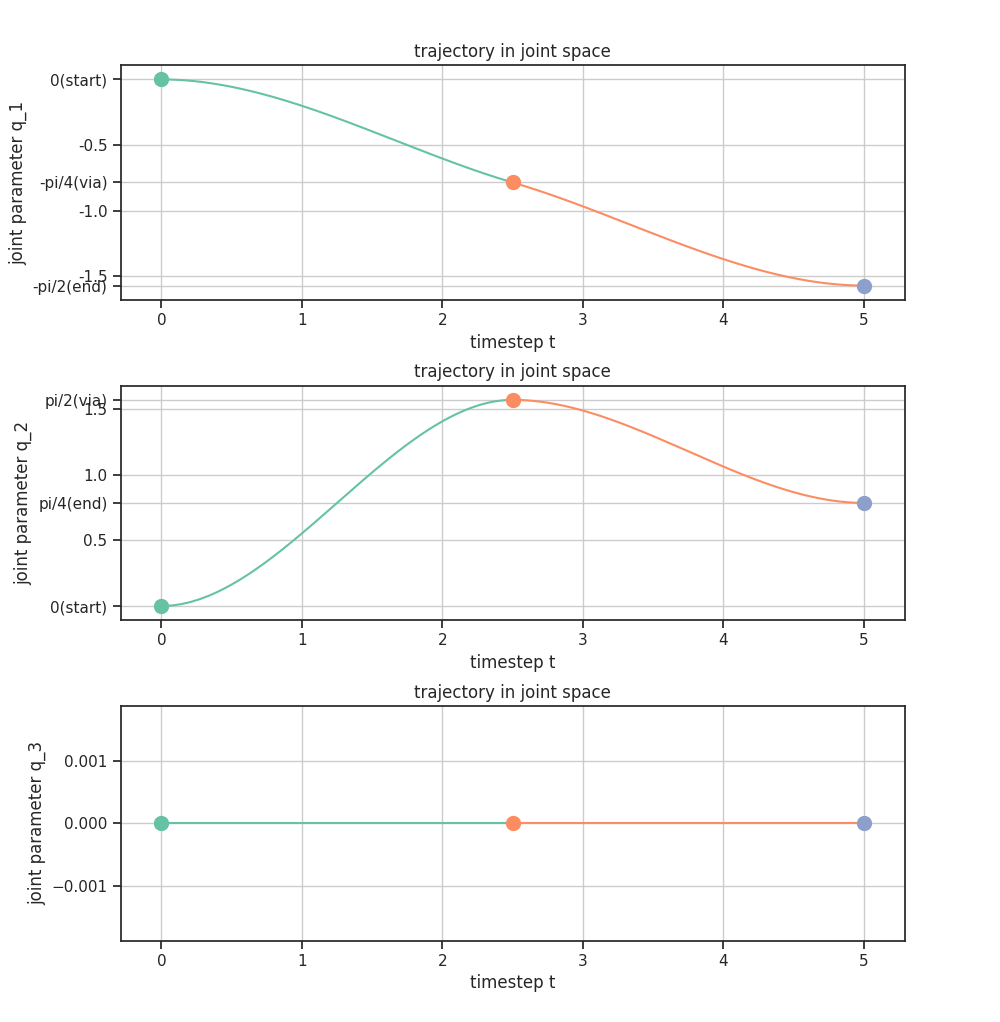
\includegraphics[scale=0.6]{../plots/B1(b)}
  \caption{joint configuration $q$ over time}
\end{figure}

% -------------------------------------

\subsection{Trajectories In Joint Space}

\setcounter{subsection}{2}
\subsection{~}

\begin{figure}[H]
  \centering
  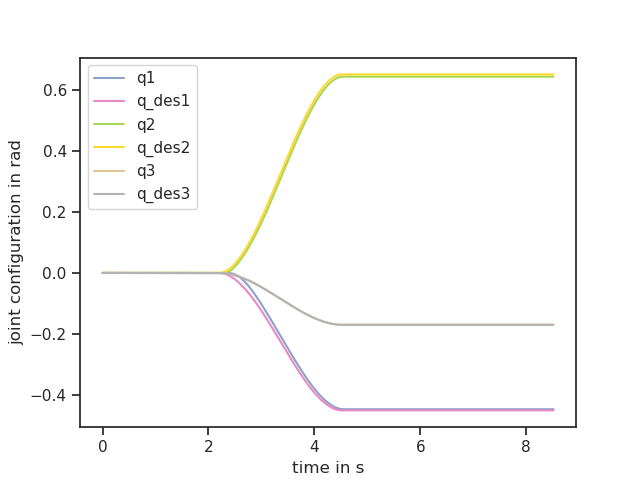
\includegraphics[scale=0.8]{img/B2_c_q}
\end{figure}

\begin{figure}[H]
  \centering
  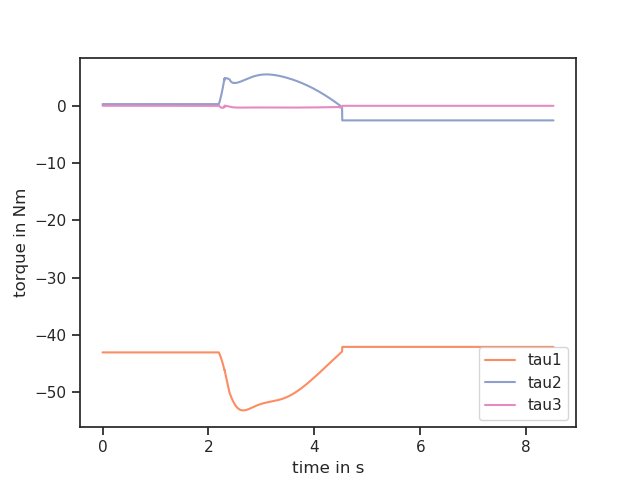
\includegraphics[scale=0.8]{img/B2_c_tau}
\end{figure}

\newpage

\section{Operational Space Control}

\setcounter{subsection}{2}
\subsection{~}

\begin{table}[h!]
  \begin{center}
    \begin{tabular}{c|c|c|c|c|c}
      \texttt{kp[0]} & \texttt{kp[1]} & \texttt{kp[2]} & \texttt{kv[0]} & \texttt{kv[1]} & \texttt{kv[2]}\\\hline
      2500 &1500 &400 &20 &100 &40 
    \end{tabular}
    \caption{our positional and velocity gains after tuning}
  \end{center}
\end{table}

\begin{figure}[H]
  \centering
  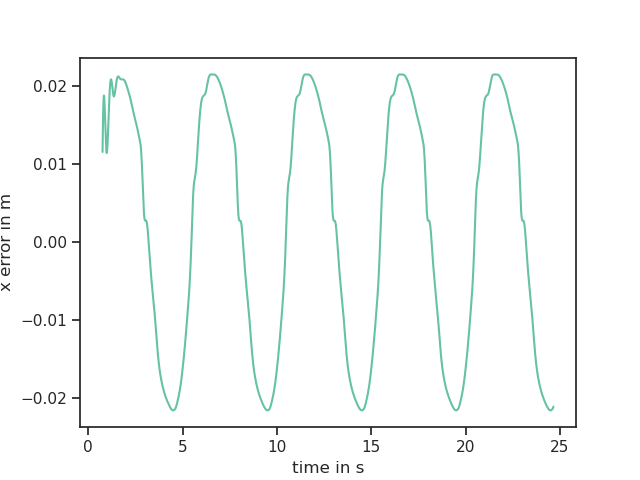
\includegraphics[scale=0.6]{img/C3_error0}
  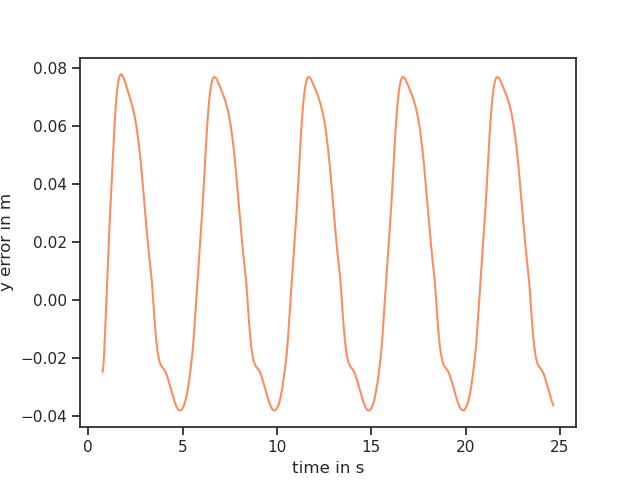
\includegraphics[scale=0.6]{img/C3_error1}
  \caption{position error $e = x - x_d$ over time}
\end{figure}

\begin{figure}[H]
  \centering
  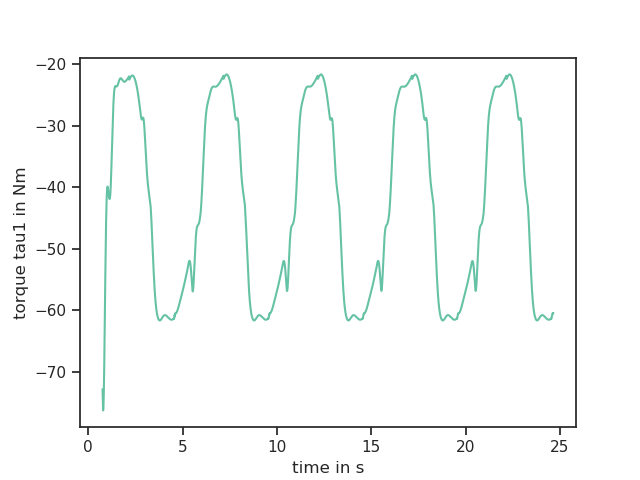
\includegraphics[scale=0.6]{img/C3_tau0}
  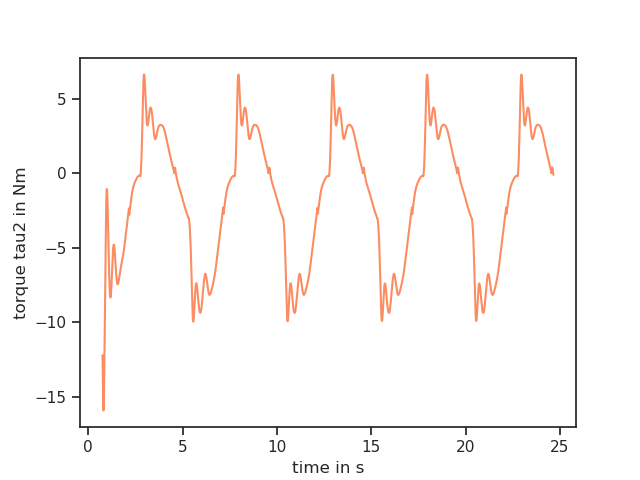
\includegraphics[scale=0.6]{img/C3_tau1}
  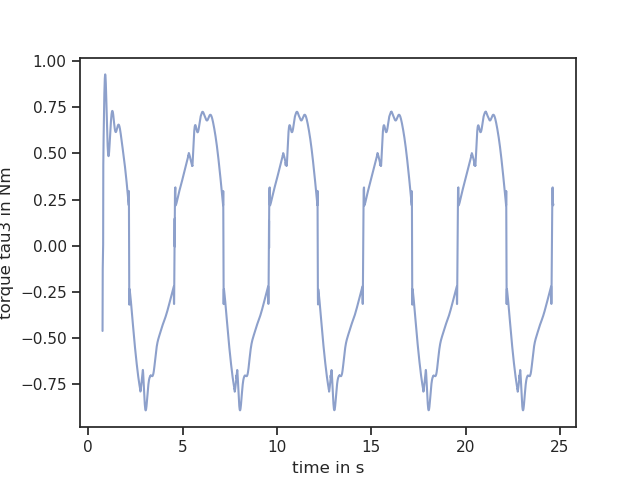
\includegraphics[scale=0.6]{img/C3_tau2}
  \caption{torque $\tau$ over time}
\end{figure}

\begin{figure}[H]
  \centering
  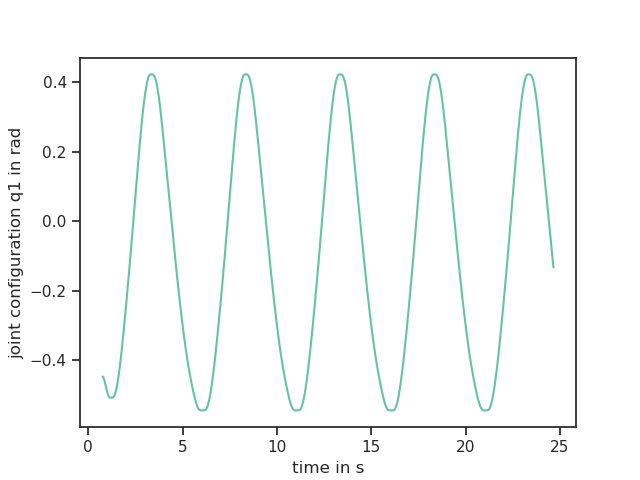
\includegraphics[scale=0.6]{img/C3_theta0}
  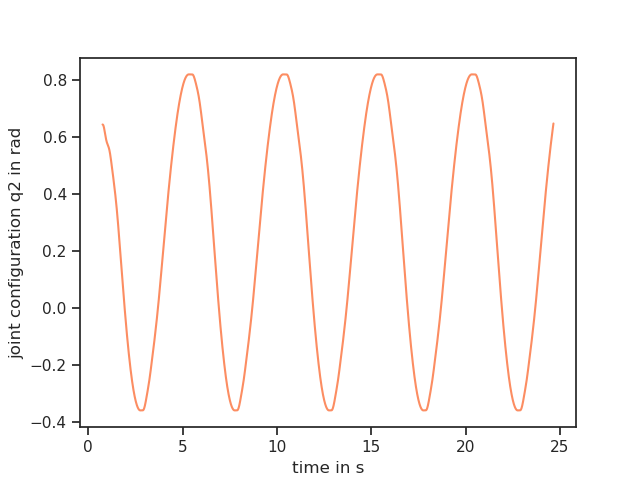
\includegraphics[scale=0.6]{img/C3_theta1}
  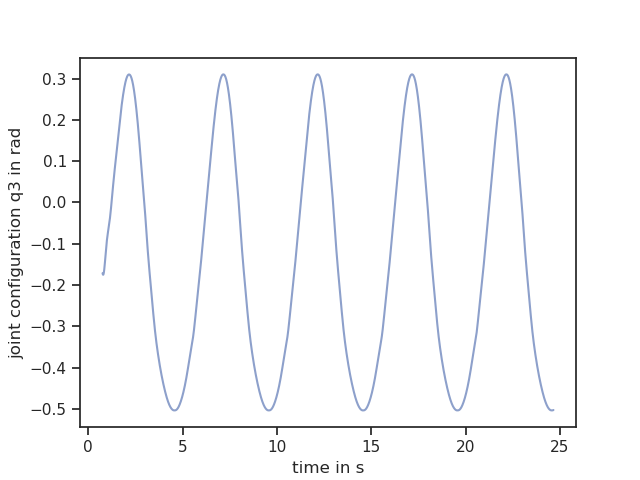
\includegraphics[scale=0.6]{img/C3_theta2}
  \caption{angle $\theta$ over time}
\end{figure}

\begin{figure}[H]
  \centering
  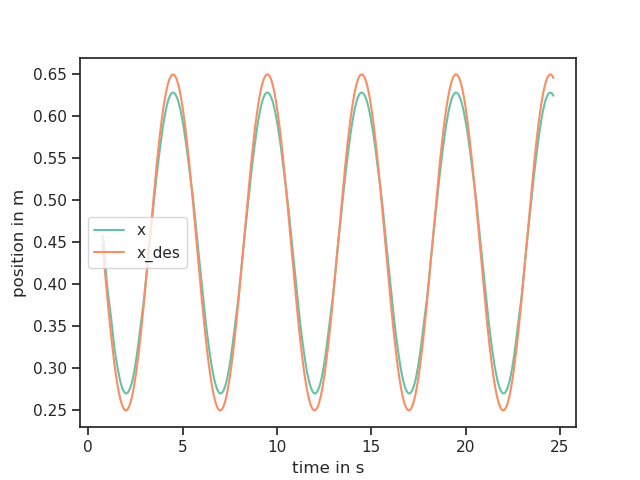
\includegraphics[scale=0.6]{img/C3_x0_xd0}
  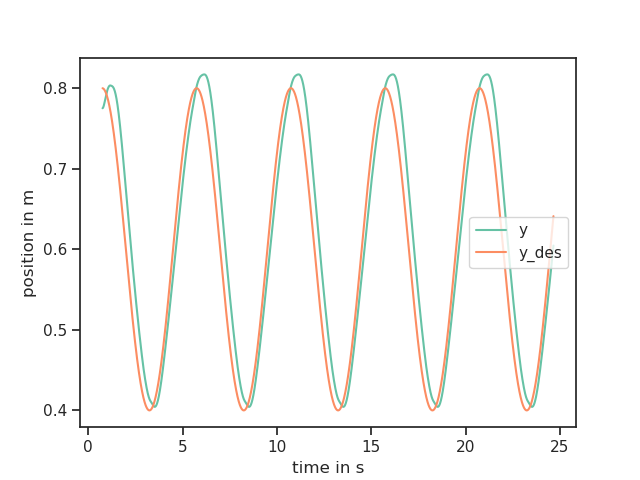
\includegraphics[scale=0.6]{img/C3_x1_xd1}
  \caption{position $x$ and desired position $x_d$ over time}
\end{figure}


\begin{figure}[H]
  \centering
  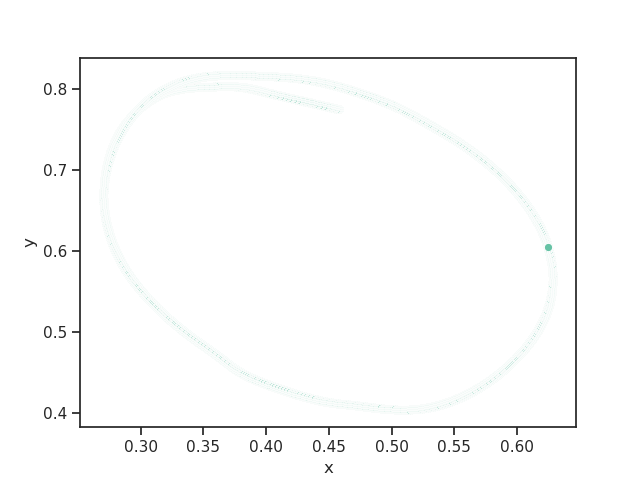
\includegraphics[scale=0.6]{img/C3_2D_plane_x}
  \caption{position $x$ in the 2D plane}
\end{figure}

\begin{figure}[H]
  \centering
  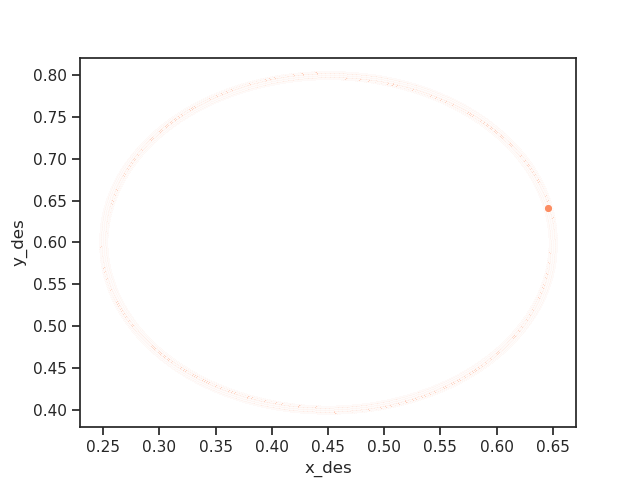
\includegraphics[scale=0.6]{img/C3_2D_plane_xd}
  \caption{desired position $x_d$ in the 2D plane}
\end{figure}

\subsection{~}

\begin{figure}[H]
  \centering
  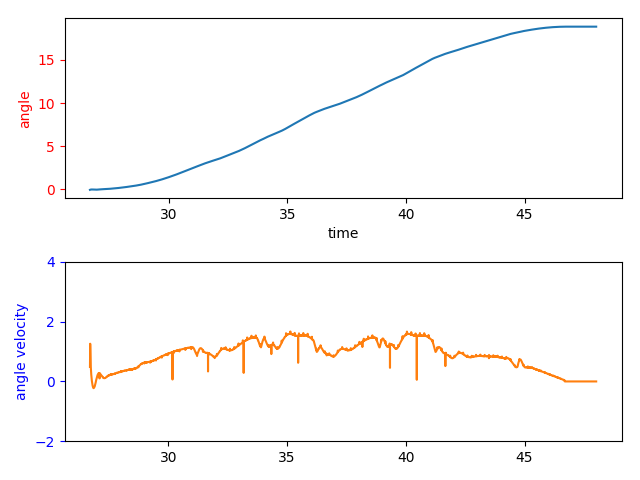
\includegraphics[scale=0.6]{img/C4}
  \caption{angle $\beta$ and angular velocity $\dot{\beta}$ over time}
\end{figure}

\end{document}
